\section{Solving Linear Equations with Iterative Solvers and the Multigrid Technique}
\thispagestyle{plain}

\textbf{Relevance of solving linear equations for simulations}: Implicit schemes lead to linear systems of equations which we have to solve,
examples already covered are implicit Euler applied to a linear ODE in sec. \ref{sssec:implicit_euler_linear},
or to a non-linear one (the linear equation then follows from doing the implicit step
by Newton-Raphson where the Jacobian is to be inverted (sec. \ref{sssec:implicit_euler_nonlinear})),
or just recently in the diffusion equation.

Another example of a linear system we care about is solving a discretized Poisson equation.

\bluebox{Direct inversion or LU or QU decomposition of our linear system (the matrix describing it)
are often too costly, so iterative methods - methods where we construct a sequence
of approximate solutions that hopefully converge to the exact solution - are used.}

\bluebox{In the multigrid-technique, differential equations are solved using a hierarchy of discretizations.}

\subsection{Motivational Example 1: From the Poisson equation we can get a possibly big linear system}
Let us discretize the 1D Poisson equation
\begin{equation}
    \begin{gathered}
        \partial_x^2 \phi = 4\pi G \rho \rightarrow (\partial_x^2\phi) \approxeq \frac{\phi_{i+1} - 2\phi_i + \phi_{i-1}}{h^2}  \approxeq  4\pi G \rho_i \\
        i = 1,\dots,N, \quad \text{spacing } h
    \end{gathered}
\end{equation}
We write this as a matrix equation
\begin{equation}
    \mat{A} \vec{\phi} = \vec{b}, \quad \vec{\phi} = \left( \begin{array}{c} \phi_1 \\ \phi_2 \\ \vdots \\ \phi_N \end{array} \right), \quad \vec{b} = 4\pi G \vec{\rho}, \vec{\rho} = \left( \begin{array}{c} \rho_1 \\ \rho_2 \\ \vdots \\ \rho_N \end{array} \right)
\end{equation}
with in the case of periodic boundary conditions
\begin{equation}
    \mat{A} = \frac{1}{h^2} \left( \begin{array}{cccccc}
            -2 & 1 & 0 & \dots & 0 & 1 \\
            1 & -2 & 1 & 0 & \dots &  \\
            0 & 1 & -2 & 1 & 0 & \dots \\
            0 & 0 & \ddots & \ddots & \ddots & 0 \\
            0 & \dots &  & 1 & -2 & 1 \\
            1 & 0 & 0 & \dots & 1 & -2
        \end{array} \right)
\end{equation}

\problem{LU-decomposition or Gauss elimination with pivoting are generally $\mathcal{O}(N^3)$ (for such a sparse matrix we can do better though).
Imagine a discretization in 3D, then for $1000$ grid points per dimension $\mat{A}$ would be $10^9 \times 10^9$ (mind the discretization in 3D is not \textit{as} simple as in 1D).}

\subsection{Poisson equation and solving a tridiagonal system}
\subsubsection{1D heat Diffusion equation with Dirichlet boundaries in matrix form}
Consider simple heat diffusion with constant heating rate $\epsilon$.

\begin{equation}
    -D \partial_x^2 T = \epsilon
\end{equation}

so a 1D Poisson equation with constant source term $\epsilon$.

Discretized we get as before

\begin{equation}
    \frac{T_{i+1}-2T_i + T_{i-1}}{\delta^2} \approxeq -\frac{\epsilon}{D}
\end{equation}

So for a state vector

\begin{equation}
    \vec{T} = \left( \begin{array}{c} T_1 \\ T_2 \\ \vdots \\ T_N \end{array} \right)
\end{equation}

with Dirichlet boundary conditions $T_1 = T_N := T_0$ we get the matrix equation

\begin{equation}
    \mat{A} \vec{T} = \vec{b}, \quad \vec{b} = \left( \begin{array}{c} T_0 \\ -\frac{\delta^2 \epsilon}{D} \\ \vdots \\ -\frac{\delta^2 \epsilon}{D} \\ T_0 \end{array} \right), \quad \mat{A} = \frac{1}{h^2} \left( \begin{array}{cccccc}
        1 & 0 & 0 & \dots & 0 & 0 \\
        1 & -2 & 1 & 0 & \dots &  \\
        0 & 1 & -2 & 1 & 0 & \dots \\
        0 & 0 & \ddots & \ddots & \ddots & 0 \\
        0 & \dots &  & 1 & -2 & 1 \\
        0 & 0 & 0 & \dots & 0 & 1
    \end{array} \right)
\end{equation}

\greenbox{So for a 1D Poisson problem with Dirichlet (constant) boundary conditions we get a tridiagonal matrix.}

\subsubsection{Forward elimination backward substitution method for solving a tridiagonal system}
Consider the general tridiagonal matrix
\begin{equation}
    \mat{A} = \left( \begin{array}{cccccc}
        d_1 & u_1 & 0 & \dots & 0 & 0 \\
        l_1 & d_2 & u_2 & 0 & \dots &  \\
        0 & l_2 & d_3 & u_3 & 0 & \dots \\
        0 & 0 & \ddots & \ddots & \ddots & 0 \\
        0 & \dots &  & l_{N-2} & d_{N-1} & u_{N-1} \\
        0 & 0 & \dots & 0 & l_{N-1} & d_N
    \end{array} \right)
\end{equation}
where we want to solve
\begin{equation}
    \mat{A} \vec{x} = \vec{b}
\end{equation}
for $\vec{x}$.
We use elementary operations $\mat{E}_i$ to add multiples of rows in $\mat{A}$ to other rows in $\mat{A}$.
\begin{enumerate}
    \item (\textcolor{blue1}{Forward elimination}) Using those operations, we succesively (top-down) eliminate the
    lower diagonal $\vec{l}$ of $\mat{A}$.
    \begin{equation}
        \mat{E}_1 \mat{E}_2 \dots \mat{E}_{N-1} \mat{A} \vec{x} = \left( \begin{array}{cccccc}
            d_1 & u_1 & 0 & \dots & 0 & 0 \\
            0 & \tilde{d}_2 & u_2 & 0 & \dots &  \\
            0 & 0 & \tilde{d}_3 & u_3 & 0 & \dots \\
            0 & 0 & \ddots & \ddots & \ddots & 0 \\
            0 & \dots &  & 0 & \tilde{d}_{N-1} & u_{N-1} \\
            0 & 0 & \dots & 0 & 0 & \tilde{d}_N
        \end{array} \right) \vec{x} = \mat{E}_1 \mat{E}_2 \dots \mat{E}_{N-1} \vec{b}
    \end{equation}
    with $\tilde{d}_2 = d_2 - \frac{l_1}{d_1} u_1$ and $\tilde{d}_i = d_i - \frac{l_{i-1}}{\tilde{d}_{i-1}} u_{i-1}$ for $i=3,\dots,N$.
    \item (\textcolor{blue1}{Backward substitution}) We can now solve the system starting from the last row.
\end{enumerate}

\subsection{Classical Exact Solution: LU-decomposition\skipthis}
\bluebox{\textbf{Why is it not a good idea to numerically
invert the matrix?: } While $\mat{A} \in \mathbb{R}^{N\times N}$ 
might often be sparse (e.g. a sparse Jacobian), $\mat{A}^{-1}$ is 
dense in general and our storage might not be able to handle $N^2$ 
terms of a dense inverse. This is not a problem of stability - the 
inverse can be computed as numerically stable as other methods are. 
Matrix inversion can even by done in $\mathcal{O}(N^{\log_2 7})$ 
(Strassen algorithm, \textit{Gaussian elimination is not optimal}).}

Let us discuss LU-decomposition (also called LR-decomposition).

Consider $\mat{L}, \mat{R} \in \mathbb{R}^{N\times N}$ and $\mat{A} \in \mathbb{R}^{N\times N}$ invertible with
\begin{equation}
    \mat{A} = \mat{L} \mat{R}, \quad \text{lower-left triangular matrix } \mat{L}, \text{ upper-right triangular matrix } \mat{R}
\end{equation}
\note{More generally, $\mat{P} \mat{A} = \mat{L} \mat{R}$ with $\mat{P}$ a permutation matrix is possible for
every invertible matrix $\mat{A}$. Otherwise the decomposition is not always possible, e.g. for $a_{11} = 0 \rightarrow l_{11}$ or $l_{11} = 0$, so
$\mat{L}$ or $\mat{R}$ would be singular (not full rank), so $\mat{A}$ would not be invertible (contradiction). So $\mat{P}$ is used to switch rows of $\mat{A}$.}

\subsubsection{Solving the linear system for $\vec{x}$ when we already know the LU-decomposition}
We can split
\begin{equation}
    \mat{A} \vec{x} = \mat{L} \mat{R} \vec{x} \quad \leftrightarrow \quad \mat{L} \vec{y} = \vec{b}, \quad \mat{R} \vec{x} = \vec{y}
\end{equation}
so into solving two triangular systems.
\begin{enumerate}
    \item (\textcolor{blue1}{Forward substitution}) Solve $\mat{L} \vec{y} = \vec{b}$ for $\vec{y}$. We can write the system as
    \begin{equation}
        \left(\begin{array}{ll}
        l_{11} & \\
        \vec{L}_{* 1} & \mat{L}_{* *}
        \end{array}\right)\left(\begin{array}{l}
        y_1 \\
        \vec{y}_*
        \end{array}\right)=\left(\begin{array}{l}
        b_1 \\
        \vec{b}_*
        \end{array}\right) \Rightarrow l_{11} y_1=b_1, \quad \vec{L}_{* 1} y_1+\mat{L}_{* *} \vec{y}_*=b_*
    \end{equation}
    from which we can solve for $y_1 = \frac{b_1}{l_{11}}$. We can then construct a new triangular
    system for $\vec{y}_*$
    \begin{equation}
        \mat{L}_{* *} \vec{y}_* = \vec{b}_* - \vec{L}_{* 1} y_1
    \end{equation}
    so $\vec{y}$ can be solved recursively, yielding the explicit formula
    \begin{equation}
        y_i=\frac{1}{l_{i i}}\left(b_i-\sum_{k=1}^{i-1} l_{i k} y_k\right)
    \end{equation}
    taking $\mathcal{O}(N^2)$ operations.
    \item (\textcolor{blue1}{Backward substitution}) Then $\mat{R} \vec{x} = \vec{y}$ for $\vec{x}$. The logic is the same as for forward substitution, 
    but bottom-up. We can write the system as
    \begin{equation}
        \left(\begin{array}{ll}
        \mat{R}_{* *} & \vec{R}_{* n} \\
        & r_{n n}
        \end{array}\right)\left(\begin{array}{l}
        \vec{x}_* \\
        x_1
        \end{array}\right)=\left(\begin{array}{l}
        \vec{y}_* \\
        y_n
        \end{array}\right)
    \end{equation}
    yielding the explicit formula
    \begin{equation}
        a_i=\frac{1}{r_{i i}}\left(y_i-\sum_{k=i+1}^N r_{i k} a_k\right)
    \end{equation}
    also taking $\mathcal{O}(N^2)$ operations.
\end{enumerate}

\subsubsection{Calculating the LU-decomposition in $\mathcal{O}(N^3)$}
From
\begin{equation}
    \left(\begin{array}{ll}
    a_{11} & \vec{A}^T_{1 *} \\
    \vec{A}_{* 1} & \mat{A}_{* *}
    \end{array}\right)=\left(\begin{array}{ll}
    l_{11} & \\
    \vec{L}_{* 1} & \mat{L}_{* *}
    \end{array}\right)\left(\begin{array}{ll}
    r_{11} & \vec{R}^T_{1 *} \\
    & \mat{R}_{* *}
    \end{array}\right), \quad \text { set diagonal of } \mat{L} \text { to } 1 \rightarrow \text { unique decomp }
\end{equation}
we can devise an $\mathcal{O}(N^3)$ algorithm to calculate $\mat{L}$ and $\mat{R}$,
see code \ref{code:lu_decomposition}.

\begin{codebox}[!htb]
    \begin{minted}{julia}
        # in-place decomposition of A into L and R, the upper-right part of A is overwritten by R,
        # the lower-left part of A is overwritten by L without diagonal (set to 1)
        function lu_decomposition!(A::Matrix{T}) where T <: Number
            N = size(A, 1)
            for i in 1:N
                for j in i+1:N
                    A[j, i] /= A[i, i]
                    for k in i+1:N
                        A[j, k] -= A[j, i] * A[i, k]
                    end
                end
            end
        end
        # one can then extract L = tril(A, -1) + I
        # and U = triu(A) via the LinearAlgebra package
    \end{minted}
    \caption{LU-decomposition of a matrix $\mat{A} \in \mathbb{R}^{N\times N}$ in $\mathcal{O}(N^3)$.}
    \label{code:lu_decomposition}
\end{codebox}

\note{Blocked versions can be parallelized, QR-decomposition retains the condition number of $\mat{A}$.}

\problem{LU-decomposition is $\mathcal{O}(N^3)$.}

\subsection{Jacobi iteration | a splitting method}
\bluebox{\textbf{Aim:} We want quicker than $\mathcal{O}(N^3)$, approximate solutions to linear systems.}

Consider the linear system
\begin{equation}
    \mat{A} \vec{x} = \vec{b}, \quad \mat{A} \in \mathbb{R}^{N\times N}, \vec{x}, \vec{b} \in \mathbb{R}^N
\end{equation}
For Jacobi iteration, we start with the trivial decomposition
\begin{equation}
    \begin{gathered}
        \mat{A} = \mat{D} - (\mat{L} + \mat{U}), \quad \text{diagonal part } \mat{D}, \quad \text{negative left-below-diagonal part} \mat{L} \\
        \text{negative right-above-diagonal part} \mat{U}
    \end{gathered}
\end{equation}
so
\begin{equation}
    \mat{A}\vec{x} = \left[ \mat{D} - (\mat{L} + \mat{U}) \right] \vec{x} = \vec{b} \quad \rightarrow \quad \vec{x} = \mat{D}^{-1} \vec{b} + \mat{D}^{-1} (\mat{L} + \mat{U}) \vec{x}
\end{equation}
so $\vec{x}$ is a fixed point of the RHS, leading to fixed-point, here \textcolor{blue1}{Jacobi iteration}
\begin{equation}
    \boxed{\vec{x}^{(n+1)} = \mat{D}^{-1} \vec{b} + \mat{D}^{-1} (\mat{L} + \mat{U}) \vec{x}^{(n)}, \quad (\mat{D}^{-1})_{ii} = \frac{1}{A_{ii}}}
\end{equation}

\subsubsection{When does the Jacobi iteration converge?}
The Jacobi iteration converges if and only if all eigenvalues $\lambda_i$ of the convergence
matrix
\begin{equation}
    \mat{M} := \mat{D}^{-1} (\mat{L} + \mat{U})
\end{equation}
are smaller than one.
\begin{equation}
    \text{spectral radius } \rho_s(\mat{M}) \equiv \max_i{|\lambda_i|} < 1
\end{equation}
\greenbox{The smaller the spectral radius, the faster the convergence.}
\subsubsubsection{Derivation of the convergence criterion}
Consider the error at step $n+1$
\begin{equation}
    \begin{gathered}
        \vec{e}^{(n+1)} = \vec{x}_{\text{exact}} - \vec{x}^{(n+1)} \underbrace{=}_{\text{Jacobi-Iteration}} \vec{x}_{\text{exact}} - \left( \mat{D}^{-1} \vec{b} + \mat{M} \vec{x}^{(n)} \right) \\
    \underbrace{=}_{\vec{x}_{\text{exact}} = \mat{D}^{-1}\vec{b}+\mat{M}\vec{x}_{\text{exact}}} \mat{M} (\vec{x}_{\text{exact}} - \vec{x}^{(n)}) = \mat{M} \vec{e}^{(n)}
    \end{gathered}
\end{equation}

so
\begin{equation}
    \vec{e}^{(n)} = \mat{M}^n \vec{e}^{(0)}
\end{equation}
which scales with $\rho_s^n(\mat{M})$ for $n$ sufficiently large (follows from decomposing $\vec{e}^{(0)}$ into eigenvectors of $\mat{M}$)
so the convergence criterion follows.

\problem{The convergence is usually slow, better use Gauss-Seidel iteration.}

\subsubsection{Example Jacobi Step}
Consider
\begin{equation}
    \mat{A} \vec{x} = \begin{pmatrix} 10 & -5 & 0 \\ -5 & 10 & -5 \\ 0 & -5 & 5 \end{pmatrix} \left( \begin{array}{c} x_1 \\ x_2 \\ x_3 \end{array} \right) = \vec{b} = \left( \begin{array}{c} 0 \\ 0 \\ 15 \end{array} \right)
\end{equation}
then
\begin{equation}
    \mat{D} = \begin{pmatrix} 10 & 0 & 0 \\ 0 & 10 & 0 \\ 0 & 0 & 5 \end{pmatrix}, \quad \mat{L} = \begin{pmatrix} 0 & 0 & 0 \\ 5 & 0 & 0 \\ 0 & 5 & 0 \end{pmatrix}, \quad \mat{R} = \begin{pmatrix} 0 & 5 & 0 \\ 0 & 0 & 5 \\ 0 & 0 & 0 \end{pmatrix}
\end{equation}
so
\begin{equation}
    \vec{x}^{(0)} = \left( \begin{array}{c} 0 \\ 0 \\ 0 \end{array} \right) \quad \rightarrow \quad \vec{x}^{(1)} = \left( \begin{array}{c} \frac{1}{10} b_0 + \frac{1}{10}\cdot 5 x^{(0)}_2 \\ \frac{1}{10} b_1 + \frac{1}{10}\cdot \left( 5 x^{(0)}_1 + 5 x^{(0)}_3 \right) \\ \frac{1}{5} b_1 + \frac{1}{5} \cdot 5 x^{0}_2 \end{array} \right)
\end{equation}

\subsection{Gauss-Seidel iteration | better splitting method}
\idea{In each step $\vec{x}^{(n)} \rightarrow \vec{x}^{(n + 1)}$ ($\vec{x} \in \mathbb{R}^N$)
consists of $N$ scalar updates. If we do these $N$ scalar updates iteratively (not in parallel)
we can use the results from previous updates.}
\subsubsection{Motivational Example}
For instance in the example above
\begin{equation}
    \vec{x}^{(0)} = \left( \begin{array}{c} 0 \\ 0 \\ 0 \end{array} \right) \quad \rightarrow \quad \vec{x}^{(1)} = \left( \begin{array}{c} \frac{1}{10} b_0 + \frac{1}{10}\cdot 5 x^{(0)}_2 \\ \frac{1}{10} b_1 + \frac{1}{10}\cdot \left( 5 x^{(1)}_1 + 5 x^{(0)}_3 \right) \\ \frac{1}{5} b_1 + \frac{1}{5} \cdot 5 x^{1}_2 \end{array} \right)
\end{equation}

\subsubsection{Gauss-Seidel update}
Let us devise a different fix-point equation
\begin{equation}
    (\mat{D}-\mat{L}) \vec{x} = \mat{U} \vec{x} + \vec{b} \rightarrow \vec{x} = (\mat{D}- \mat{L})^{-1} \mat{U} \vec{x} + (\mat{D} - \mat{L})^{-1} \vec{b}
\end{equation}
from which we follow the fix-point iteration
\begin{equation}
    \vec{x}^{(n+1)} = (\mat{D} - \mat{L})^{-1} \mat{U} \vec{x}^{(n)} + (\mat{D} - \mat{L})^{-1} \vec{b}
\end{equation}
\problem{We cannot easily compute $(\mat{D} - \mat{L})^{-1}$.}
Therefore, multiply with $(\mat{D} - \mat{L})$.
\begin{equation}
    (\mat{D} - \mat{L}) \vec{x}^{(n+1)} = \mat{U} \vec{x}^{(n)} + \vec{b} \quad \rightarrow \quad \vec{x}^{(n+1)} = \mat{D}^{-1} \mat{L} \vec{x}^{(n+1)} + \mat{D}^{-1} \mat{U} \vec{x}^{(n)} + \mat{D}^{-1} \vec{b}
\end{equation}
\yellowbox{\textbf{But isn't this implicit now with $\vec{x}^{(n+1)}$ on both sides?}: $\mat{L}$ is a lower diagonal matrix (diagonal and everything above zero), so in $\mat{L} \vec{x}^{(n+1)}$ we always only need values we have already calculated if we solve consecutively ($\rightarrow$ \textcolor{red1}{problem for parallelization}).
This is illustrated in fig. \ref{fig:lower_sel}.}

\begin{figure}[H]
    \centering
    \includesvg[width=0.5\textwidth]{figures/lower_sel.svg}
    \caption{As of $\mat{L} \vec{x}^{(n+1)}$ to calculate $x^{(n+1)}_i$ we only need $x^{(n+1)}_0, \dots, x^{(n+1)}_{i-1}$ which we have already calculated.}
    \label{fig:lower_sel}
\end{figure}

\greenbox{\textbf{Advantage of Gauss-Seidel: } Convergence is sped up (often by a factor of 2) compared to Jacobi iteration. Convergence is guaranteed if $\mat{A}$ is strictly diagonally dominant $\left|A_{i i}\right| > \sum_{j \neq i}\left|A_{i j}\right| \quad \forall i$ or symmetric and positive definite.}

\subsubsection{The problem of parallelization in Gauss-Seidel and red-black ordering}
\problem{In Gauss-Seidel, the equations must be solved in sequential order - this cannot be parallelized. A general problem of using information from the same step is that the overall result is order dependent (which element is selected first).}
\idea{Do not do a scheme with sequential dependence (where information is used as soon as available) but if possible e.g. rather split the $N$ updates into two groups where
all updates within a group are independent, but the updates of the second group depend on the ones from first.}



For instance for the 2d-Poisson equation, \textit{a red-black ordering} scheme can be derived, see figure \ref{fig:red_black} (details follow).

\begin{figure}[H]
    \centering
    \includesvg[width=0.9\textwidth]{figures/red_black.svg}
    \caption{Red-black ordering for the 2D Poisson equation.}
    \label{fig:red_black}
\end{figure}

\subsection{Relaxation problem | Poisson equation in red-black ordering}
\bluebox{We can physically understand why applying an iterative scheme to a stationary (elliptic) problem
makes sense in terms of relaxation of a dynamical system.}
\subsubsection{Formulating an elliptic equation as an equilibrium of a relaxation problem}
Consider the elliptic equation
\begin{equation}
    Lx = b
\end{equation}
for instance for the gravitational 2D-Poisson problem $(\partial_x^2 + \partial_y^2) \phi = 4\pi G \rho$.

The elliptic problem can be written as the equilibrium of the relaxation problem

\begin{equation}
    \frac{1}{K} \partial_t x = L x - b, \quad \text{for } \partial_t x = 0 \text{ for } t \rightarrow \infty, \quad \text{some factor } K \text{ in } \frac{\m^2}{s}
\end{equation}

\subsubsection{Red-black ordering for the 2D Poisson equation}
Consider for instance the 2D Poisson equation, formulated as a relaxation problem, here central in space,
forward in time
\begin{equation}
    K \frac{\phi_{i, j}^{(n+1)}-\phi_{i, j}^{(n)}}{\Delta t}=\frac{\phi_{i+1, j}^{(n)}-2 \phi_{i, j}^{(n)}+\phi_{i-1, j}^{(n)}}{\Delta x^2}+\frac{\phi_{i, j+1}^{(n)}-2 \phi_{i, j}^{(n)}+\phi_{i, j-1}^{(n)}}{\Delta x^2}-4 \pi G \rho_{i j}
\end{equation}
so
\begin{equation}
    \label{eq:2dpoisson_disc}
    \phi_{i, j}^{(n+1)}=\frac{K \Delta t}{\Delta x^2}\left(\phi_{i+1, j}^{(n)}+\phi_{i-1, j}^{(n)}+\phi_{i, j+1}^{(n)}+\phi_{i, j-1}^{(n)}\right)+\underbrace{\left(1-4 \frac{K \Delta t}{\Delta x^2}\right)}_{= \, 0 \text{ by choice } \Delta t = \frac{1}{4} \frac{\Delta x^2}{K}} \phi_{i, j}^{(n)}-4 \pi G \rho_{i j} \Delta t
\end{equation}
where the time-step choice is akin to the CFL criterion in diffusion.
\greenbox{The discretized Poisson-relaxation update lends itself naturally to a red-black ordering scheme.}

\subsection{Multigrid technique}
We have now gained an understanding of iteratively
solving a linear equation as a relaxation problem.
\note{In each update step information travels as given by
the stencil, for the Poisson equation only between 
nearest neighbors. This also limits the largest
possible \textit{timestep} to the CFL criterion.}

\problem{As only cells in the stencil (often only 
neighboring cells) communicate per step
in Jacobi and Gauss-Seidel iteration, we have to make a
compromise between speed of convergence and resolution:
\begin{itemize}
    \item On a coarse grid, information travels quicker through space (in less steps) but the resolution is bad
    \item On a fine grid, resolution is good, but long range interactions take lots of computational steps and long-wavelength errors (in the error vector $\vec{e}$) die out only very slowly
\end{itemize}
}

\idea{Start on a coarse grid, where information travels quickly, long range correlations are taken care of and we have fast convergence, then get the information onto a fine grid and resolve the details.}

\begin{enumerate}
    \item But how can we map from a coarser to a finer grid and vice versa?
    \item How can we solve $\mat{A}\vec{x} = \vec{b}$ on the coarser grid?
\end{enumerate}

\note{Coarse-to-fine is called prolongation, fine-to-coarse restriction (see figure \ref{fig:pro_res_grids}).}

\begin{figure}
    \centering
    \includesvg[width=0.9\textwidth]{figures/pro_res.svg}
    \caption{Grids of different resolution.}
    \label{fig:pro_res_grids}
\end{figure}

\subsubsection{Getting finer and coarser | prolongation and restriction}

\note{In the following we will only consider the case of a 1D grid (not 2D as illustrated before).}

Consider meshes
\begin{enumerate}
    \item Let $\Omega^{(h)}$ denote a 1D mesh with $N$ cells $i=1,\dots,N$ with spacing $h$.
    \item Let $\Omega^{(2h)}$ denote a 1D mesh with $N/2$ cells $i=1,\dots,N/2$ with spacing $2h$.
\end{enumerate}
and let
\begin{enumerate}
    \item $\vec{x}^{(h)}_i \in \mathbb{R}^{N}$ denote the solution on $\Omega^{(h)}$, so $x^{(h)}_i$ is the solution on cell $i$ of $\Omega^{(h)}$ (e.g. a density $\rho^{(h)}_i$).
    \item $\vec{x}^{(2h)}_i \in \mathbb{R}^{N/2}$ denote the solution on $\Omega^{(2h)}$, so $x^{(2h)}_i$ is the solution on cell $i$ of $\Omega^{(2h)}$.
\end{enumerate}

Restriction and prolongation in 1D are illustrated in figure \ref{fig:pro_res_ill}.

Prolongation and restriction are linear operators written as matrices $\mat{I}_{\text{from this spacing}}^{\text{to this spacing}}$.

\begin{figure}[H]
    \centering
    \includesvg[width=0.5\textwidth]{figures/pro_res_ill.svg}
    \caption{Illustration of restriction and prolongation.}
    \label{fig:pro_res_ill}
\end{figure}

\subsubsubsection{Coarse-to-fine | interpolation called prolongation}
We map from coarse to fine using
\begin{equation}
    \mat{I}_{2h}^h \vec{x}^{(2h)} = \vec{x}^{(h)}
\end{equation}
for instance by
\begin{equation}
    \mat{I}_{2h}^h \in \mathbb{R}^{N \times \frac{N}{2}}: \text{for } 0 \leq i < \frac{N}{2}: x_{2i}^{(h)} = x_i^{(2h)}, \quad x_{2i+1}^{(h)} = \frac{1}{2} \left( x_i^{(2h)} + x_{i+1}^{(2h)} \right)
\end{equation}
as shown in figure \ref{fig:pro_res_ill} and furthermore in figure \ref{fig:prolongation}.

\begin{figure}[H]
    \centering
    \includesvg[width=0.9\textwidth]{figures/prolongation.svg}
    \caption{1D-Prolongation from coarse to fine grid.}
    \label{fig:prolongation}
\end{figure}

\subsubsubsection{Fine-to-coarse | restriction}
We now convert
\begin{equation}
    \mat{I}_{h}^{2h} \vec{x}^{(h)} = \vec{x}^{(2h)}
\end{equation}
with a simple example being
\begin{equation}
    \mat{I}_{h}^{2h} \in \mathbb{R}^{\frac{N}{2} \times N}: \text{for } 0 \leq i < \frac{N}{2}: x_i^{(2h)} = \frac{x_{2i-1}^{(h)} + 2x_{2i}^{(h)} + x_{2i+1}^{(h)}}{4}
\end{equation}

\subsubsubsection{Relation of restriction and prolongation}
Prolongation and restriction matrices are oftentimes constructed to be
scaled transposes of each other, so
\begin{equation}
    \mat{I}_h^{2h} = c[\mat{I}_{2h}^{h}]^T
\end{equation}

Consider for instance

\begin{equation}
    \begin{gathered}
        \text{prolongation: } \mat{I}_{2h}^{h} = \frac{1}{2}\left(\begin{array}{lll}
            1 & & \\
            2 & & \\
            1 & 1 & \\
            & 2 & \\
            & 1 & 1 \\
            & & 2 \\
            & & 1
            \end{array}\right) \\ \text{restriction: } \mat{I}_{h}^{2h} = \frac{1}{2} \left( \mat{I}_{2h}^{h} \right)^T = \frac{1}{4} \left(\begin{array}{lllllll}
                1 & 2 & 1 & & & & \\
                & & 1 & 2 & 1 & & \\
                & & & & 1 & 2 & 1
                \end{array}\right)
    \end{gathered}
\end{equation}

so the application of \textbf{prolongation} means

\begin{equation}
    \frac{1}{2}\left(\begin{array}{lll}
    1 & & \\
    2 & & \\
    1 & 1 & \\
    & 2 & \\
    & 1 & 1 \\
    & & 2 \\
    & & 1
    \end{array}\right)\left(\begin{array}{l}
    x^{(2h)}_1 \\
    x^{(2h)}_2 \\
    x^{(2h)}_3
    \end{array}\right)=\left(\begin{array}{l}
    x^{(2h)}_1 / 2 \\
    x^{(2h)}_1 \\
    x^{(2h)}_1 / 2+x^{(2h)}_2 / 2 \\
    x^{(2h)}_2 \\
    x^{(2h)}_2 / 2+x^{(2h)}_3 / 2 \\
    x^{(2h)}_3 \\
    x^{(2h)}_3 / 2
    \end{array}\right)=\left(\begin{array}{l}
    x^{(h)}_1 \\
    x^{(h)}_2 \\
    x^{(h)}_3 \\
    x^{(h)}_4 \\
    x^{(h)}_5 \\
    x^{(h)}_6 \\
    x^{(h)}_7
    \end{array}\right)
\end{equation}

and \textbf{restriction}

\begin{equation}
    \frac{1}{4}\left(\begin{array}{lllllll}
    1 & 2 & 1 & & & & \\
    & & 1 & 2 & 1 & & \\
    & & & & 1 & 2 & 1
    \end{array}\right)\left(\begin{array}{l}
    x^{(h)}_1 \\
    x^{(h)}_2 \\
    x^{(h)}_3 \\
    x^{(h)}_4 \\
    x^{(h)}_5 \\
    x^{(h)}_6 \\
    x^{(h)}_7
    \end{array}\right)=\left(\begin{array}{l}
    x^{(2h)}_1 \\
    x^{(2h)}_2 \\
    x^{(2h)}_3
    \end{array}\right)
\end{equation}

Both are illustrated in figure \ref{fig:sinprores}, also illustrating that with respect to 
the grid index, low-frequency errors on the fine grid have double (so higher) frequency on the coarse grid.

\begin{figure}[H]
    \centering
    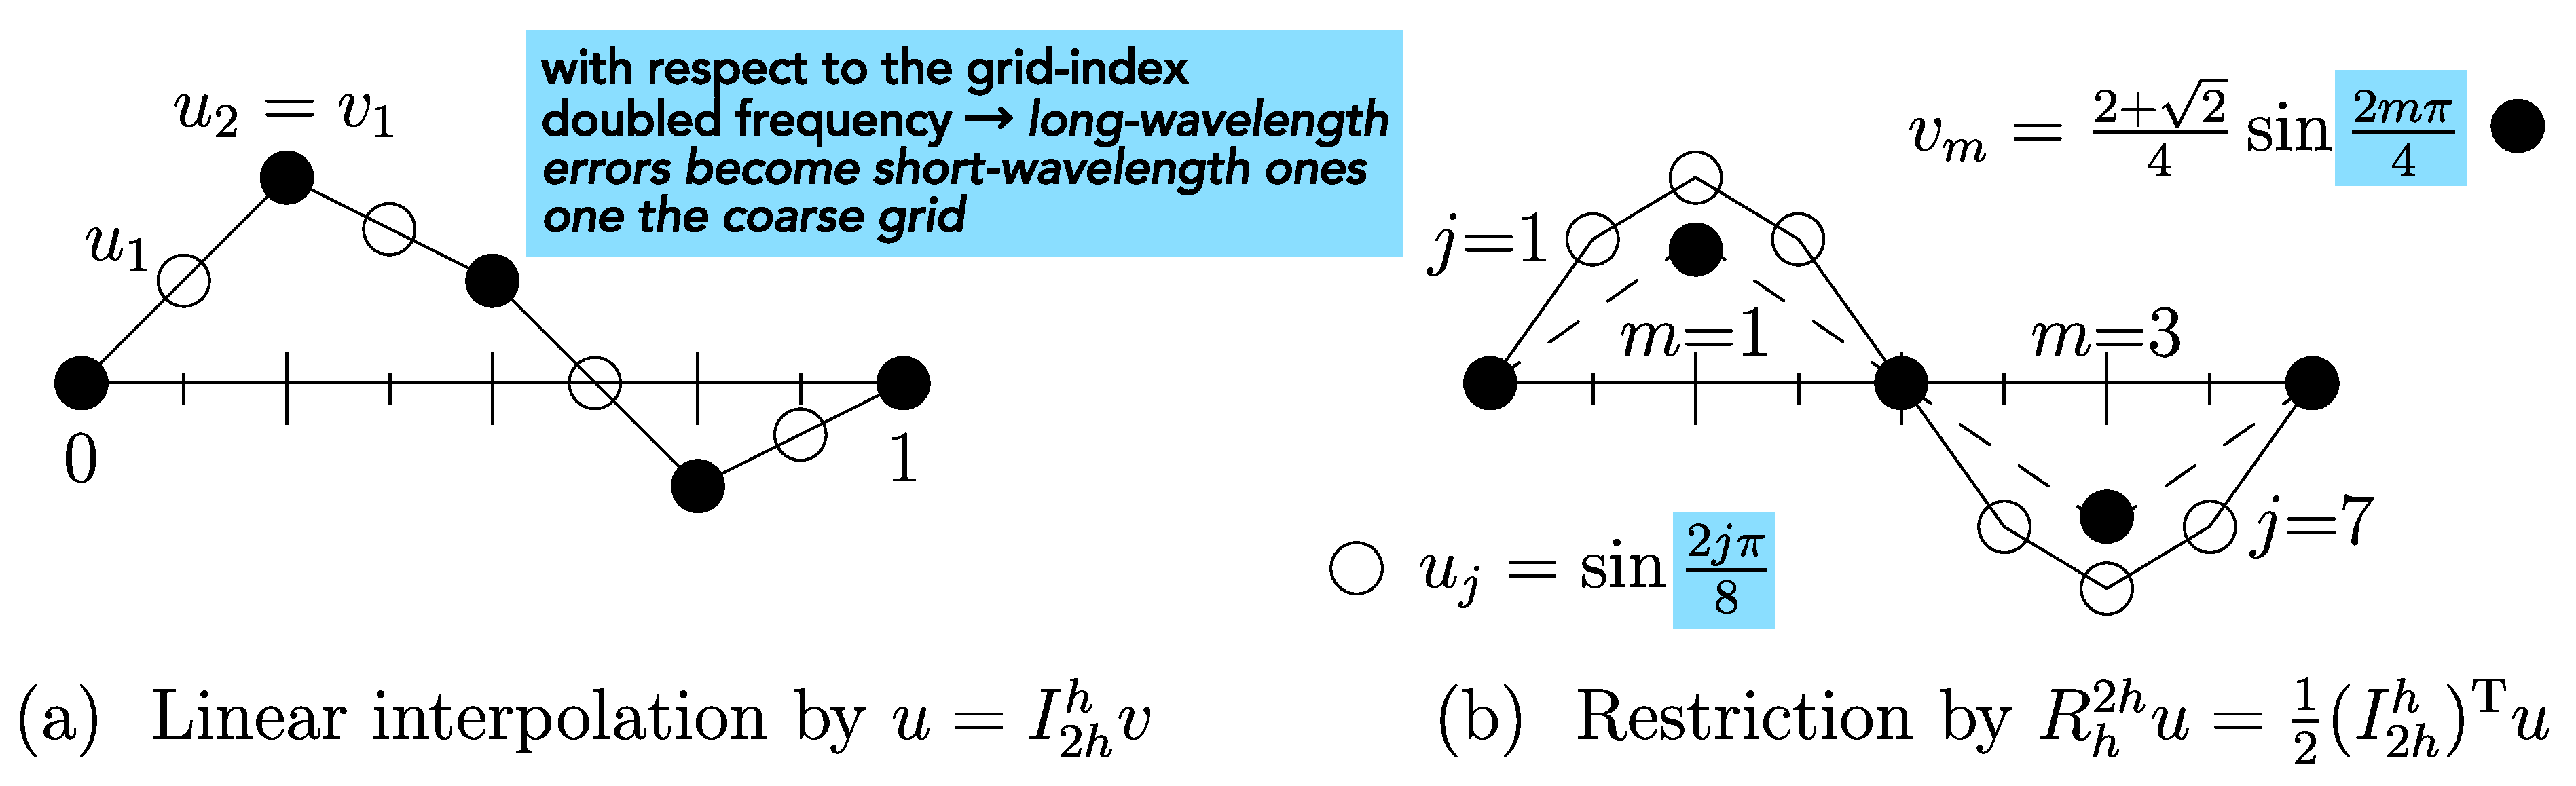
\includegraphics[width=0.9\textwidth]{figures/sinprores.pdf}
    \caption{Prolongation and restriction of a sine wave (figure by Gilbert Strang).}
    \label{fig:sinprores}
\end{figure}

\note{Taking prolongation and restriction as transposes of each others breaks at the boundaries, if we do not
as in figure \ref{fig:sinprores} have zeroes on the boundaries.}

\subsubsubsection{Short-hand stencil notation}

Short-hand notations for prolongation and restriction are
given in table \ref{tab:pro_res_short}.

\begin{table}[H]
    \centering
    \begin{tabular}{|p{0.45\textwidth}|p{0.45\textwidth}|}
        \hline
        \textbf{Prolongation} & \textbf{Restriction} \\
        \hline
        We can write prolongation as
        \begin{equation}
            \text{1D prolongation: } \mat{I}_{2h}^{h}: \left] \begin{array}{lll} \frac{1}{2} & 1 & \frac{1}{2} \end{array} \right[
        \end{equation}
        meaning that every coarse point is added to three fine points with these respective weights (see previous example). &
        We can write restriction as
        \begin{equation}
            \text{1D restriction: } \mat{I}_{h}^{2h}: \left[ \begin{array}{lll} \frac{1}{4} & \frac{1}{2} & \frac{1}{4} \end{array} \right]
        \end{equation}
        - the coarse point is the weighted sum of the three fine points. \\
        \hline
    \end{tabular}
    \caption{Short-hand notations for prolongation and restriction.}
    \label{tab:pro_res_short}
\end{table}

Similar short-hand notations can be devised for 2D and 3D.

\subsubsection{Multigrid V-cycle}
Our aim is still to solve $\mat{A}\vec{x} = \vec{b}$ smartly, by - in the view
of a relaxation problem - doing the rough large-scale work quickly on a coarse
and the fine details on a fine grid afterwards. We still have to anwer
\begin{itemize}
    \item How can such a procedure look like?
    \item How do we convert $\mat{A}$ to coarser grids?
\end{itemize}

\subsubsubsection{Initial definitions}
The error is defined as
\begin{equation}
    \vec{e} \equiv \vec{x}_{\text{exact}} - \vec{\tilde{x}}, \quad \text{current approximate solution } \vec{\tilde{x}}
\end{equation}

\note{The residual is the error in the solution, not $\vec{x}$. The error and residual are related linearly by $\mat{A}$.
\begin{equation}
    \mat{A} \vec{x}_{\text{exact}} = \vec{b} \quad \rightarrow \quad \mat{A} (\vec{e} + \vec{\tilde{x}}) = \vec{b} \quad \rightarrow \quad \mat{A} \vec{e} = \vec{r}
\end{equation}}

\idea{Consider we have an initial guess $\vec{\tilde{x}}$ on the fine grid. We can easily calculate the residual $\vec{r}$.
We can then restrict $\vec{r}$ to a coarse grid, solve for the error there ($\mat{A} \vec{e} = \vec{r}$) (given we can transform $\mat{A}$ to the coarse grid)
and then prolong the error to the fine grid and make the correction $\vec{x}_{\text{exact}} = \vec{\tilde{x}} + \vec{e}$.}

Let us formalize this idea.

\subsubsubsection{Coarse-grid correction scheme}
\bluebox{We use the error calculated on the coarse grid to correct on the fine grid.}
Let us start with a (fine-grid) guess $\vec{\tilde{x}}^{(h)}$ for the problem
\begin{equation}
    \mat{A}^{(h)} \vec{x}^{(h)} = \vec{b}^{(h)}
\end{equation}
and we want to obtain an improvement $\vec{\tilde{x}'}^{(h)} = CG(\vec{\tilde{x}}^{(h)}, \vec{b}^{(h)})$.

$CG$ consists of the following steps
\begin{enumerate}
    \item Perform \textcolor{blue1}{one iterative \textit{relaxation}} step on the current grid $h$, e.g. Jacobi or Gauss-Seidel
    \item \textcolor{blue1}{Compute the residual}
    \begin{equation}
        \vec{r}^{(h)} = \vec{b} - \mat{A}\vec{\tilde{x}}^{(h)}
    \end{equation}
    \item \textcolor{blue1}{Restrict the residual} to the coarser mesh
    \begin{equation}
        \vec{r}^{(2h)} = \mat{I}_{h}^{2h}\vec{r}^{(h)}
    \end{equation}
    \item \textcolor{blue1}{Solve for the error on the coarser mesh}
    \begin{equation}
        \mat{A}^{(2h)}\vec{e}^{(2h)} = \vec{r}^{(2h)}, \quad \text{starting guess } \vec{\tilde{e}}^{(2h)} = \vec{0}
    \end{equation}
    \item \textcolor{blue1}{Correct $\vec{\tilde{x}}^{(h)}$ on the finer mesh} using the prolonged error
    $\vec{e}^{(h)} = \mat{I}_{2h}^{h} \vec{e}^{2h}$
    \begin{equation}
        \vec{\tilde{x}'}^{(h)} = \vec{\tilde{x}}^{(h)} + \vec{e}^{(h)}
    \end{equation}
    \item \textcolor{blue1}{Further iterative \textit{relaxation}} step on the fine mesh
\end{enumerate}

\bluebox{\textbf{How to solve for the error on the coarse mesh?: } Step 4 can be performed by 
recursively calling $CG(\vec{\tilde{x}}^{(2^ih)}, \vec{b}^{(2^ih)}), i\geq 1$ until 
a coarseness is reached where one can easily exactly solve or solve by multiple relaxation
steps.}

\bluebox{\textbf{How to find $\mat{A}^{(2h)}$ on the coarse mesh?: } Generally
in the \textbf{Galerkin coarse grid approximation} one defines
\begin{equation}
    \mat{A}^{(2h)} = \mat{I}_h^{2h} \mat{A}^{(h)} \mat{I}_{2h}^{h}
\end{equation}
which is an \textcolor{red1}{additional matrix operation that might enlarge the stencil (and so the computational cost), 
depending on the interpolation operator}. 

When $\mat{A}$ was brought forth by formulating a discretization in matrix form, we can
use the same discrete equations as one the fine grid (\textbf{direct method}). In other words, the same
stencil (\textit{Schablone}) is used to go over the points and collect for the linear relations,
e.g. for the 2D-Poisson - no matter the coarseness - we would construct $\mat{A}$ based on eq. \ref{eq:2dpoisson_disc}.}

\subsubsubsection{V-cycle}
The 6-step iteration process with a recursion call in step 4 leads to a cycle as
illustrated in figure \ref{fig:vcycle}.

\begin{figure}[H]
    \centering
    \includesvg[width=0.9\textwidth]{figures/vcycle2.svg}
    \caption{V-cycle.}
    \label{fig:vcycle}
\end{figure}

The V-cycle for the Poisson equation has the same cost as FFT-based methods but
requires less thread communication when parallelized.

\bluebox{\textbf{Computational costs}
\begin{equation}
    \begin{gathered}
        \text{computational cost per V-cycle:} \mathcal{O}(N_{\text{grid}}) \\
        \text{computational cost until convergence to machine error (mult. cycles) } \mathcal{O}(N_{\text{grid}} \log{N_{\text{grid}}}) \\
        \text{with } N_{\text{grid}} \text{ being the number of grid-cells on the fine grid} \\
    \end{gathered}
\end{equation}
}

\subsubsubsection{Full multigrid method}
\problem{How to make a good initial guess $\vec{\tilde{x}}^{(h)}$ (if not available e.g. by taking the result from
the last time-step in a simulation)?}
\idea{First solve on the coarsest grid, then interpolate up to get a good initial guess. Based on this
idea, the \textcolor{blue1}{full multigrid cycle} is constructed.}

The multigrid cycle is illustrated in figure \ref{fig:full_multigrid}.

\begin{figure}[H]
    \centering
    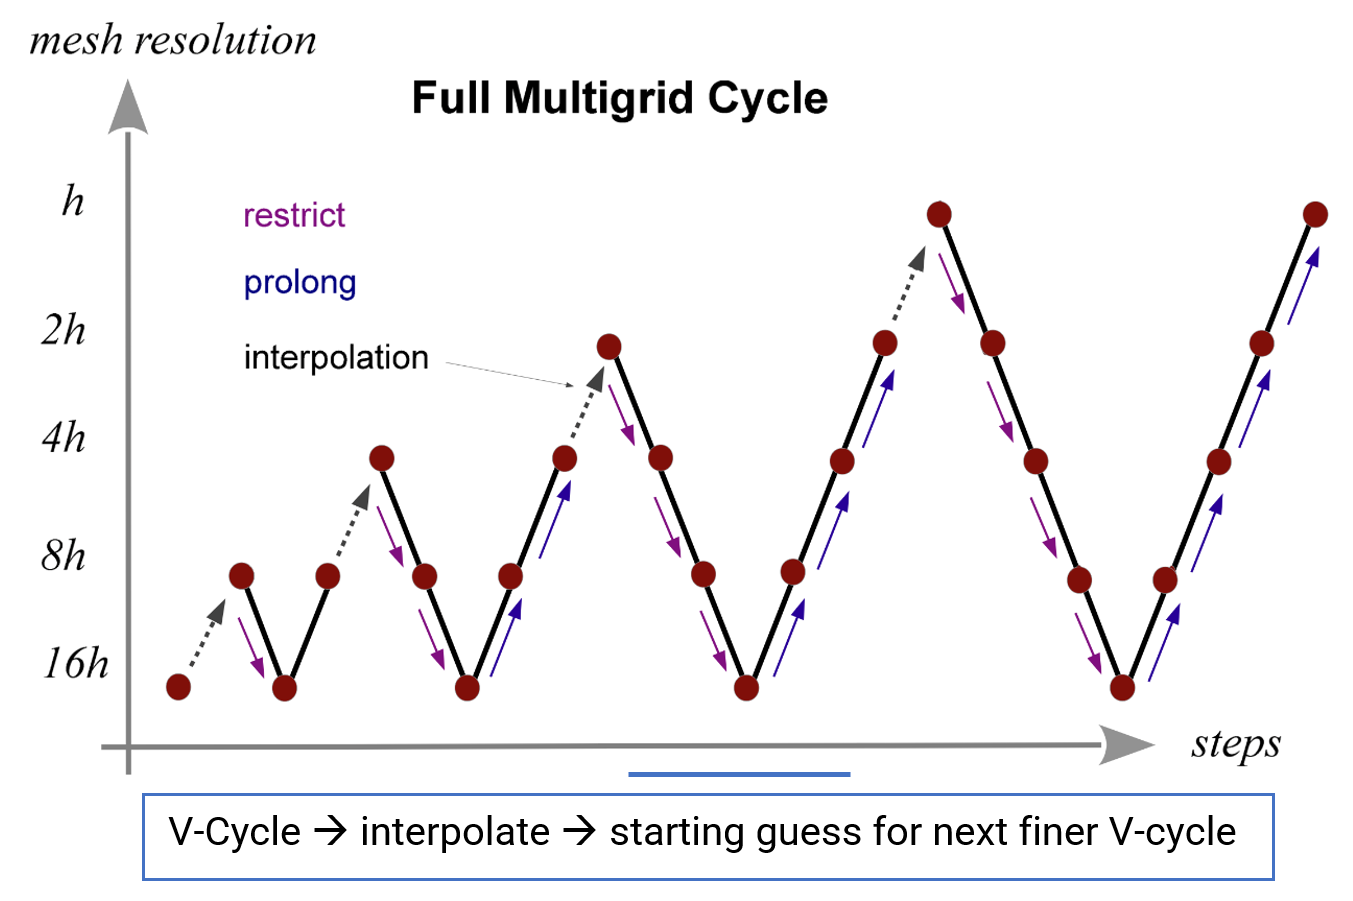
\includegraphics[width=0.9\textwidth]{figures/multigrid_cycle.png}
    \caption{Full multigrid cycle.}
    \label{fig:full_multigrid}
\end{figure}

The steps are
\begin{enumerate}
    \item Initialize the righthand side on all grid levels $\vec{b}^{(h)}, \vec{b}^{(2h)}, \vec{b}^{(H)}$.
    \item Solve $A^{(H)} \vec{x}^{(H)} = \vec{b}^{(H)}$ exactly on the coarsest level $H$.
    \item Obtain an initial guess for a finer grid by interpolating the solution from the next coarser level below, i.e. $\vec{\tilde{x}}^{(h)} = \mat{I}_{2h}^{h} \vec{\tilde{x}}^{(2h)}$
    \item Solve the problem in the finer level using this starting guess $\vec{\tilde{x}}^{(h)}$ and \textcolor{blue1}{one v-cycle}.
    \item repeat step 3 until finest level is reached
\end{enumerate}

\bluebox{\textbf{Computational cost of one multigrid cycle: } As the V-cycle it has $\mathcal{O}(N_\text{grid})$ as $N_\text{grid}$ is large compared to the cost of the V-cycle hierarchy.}

\subsection{Krylow subspace methods}
Our aim still is to solve a linear system $\mat{A}\vec{x} = \vec{b}$.

\problem{LU-decomposition has cubic runtime ($\sim \frac{2}{3} n^3$) and the previously discussed iterative methods might
also not always be optimal.}

\subsubsection{Motivation for the need of Krylow subspace methods in the context of non-linear root-finding of big systems\skipthis}
Consider a non-linear equation
\begin{equation}
    \vec{0} = g(\vec{\xi})
\end{equation}
which we want to solve for $\xi$.\footnote{For instance an implicit Euler
step can be formulated as such a root finding problem.
\begin{equation}
    \begin{gathered}
        \text{implicit step } \vec{y}^{(n+1)}=\vec{y}^{(n)}+\Delta t \vec{f}\left(\vec{y}^{(n+1)}\right) \\
        \rightarrow \quad \text{root-finding-problem } \vec{0}=\mathcolor{green1}{\vec{y}^{(n+1)}}-\vec{y}^{(n)}-\Delta t \vec{f}\left(\mathcolor{green1}{\vec{y}^{(n+1)}}\right)=: \vec{g}(\mathcolor{green1}{\vec{\xi}})
    \end{gathered}
\end{equation}}
A common root-finding approach is Newton-Iteration\footnote{Which has quadratic convergence - as the method converges on the root, the difference between the root and the approximation is squared in each step.}
\begin{equation}
    \vec{\xi}_{k+1} = \xi_{k} - \mat{J}_g^{-1} (\vec{\xi}_k) g(\vec{\xi}_k), \quad \text{Jacobian } \mat{J}_g
\end{equation}
where at the lowest level we have to solve the linear equation
\begin{equation}
    \vec{b} := \vec{g}(\vec{\xi}_k) = \mat{J}_\vec{g} \mathcolor{green1}{(\vec{\xi}_k - \vec{\xi}_{k+1})} = \mat{J}_\vec{g} \mathcolor{green1}{\vec{a}}
\end{equation}
for $\mathcolor{green1}{\vec{a}}$.
\problem{But what if the resulting Jacobian is too large to be stored?}
\idea{A directional derivative (a Jacobian vector product\footnote{\begin{equation}\begin{gathered}
    \mat{J} \vec{v}=(\vec{\nabla} \cdot \vec{g}) \vec{v}=\lim _{h \rightarrow 0} \frac{g(\vec{x}+\vec{v} h)-g(\vec{x})}{h} \\
    \left(\text{as } (\mat{J} \vec{v})_i=\sum_{j=1}^n\left(\mat{J}_g\right)_{i j} v_j=\sum_{j=1}^n \frac{\partial g_i}{\partial x_j} v_j=((\vec{\nabla} \cdot \vec{g}) \vec{v})_i\right)
    \end{gathered}\end{equation}}) can be calculated in one (forward) automatic differentiation pass - cheaply and storage efficient. So what if
we could solve $\mat{J}\vec{a} = \vec{b}$ only based on Jacobian vector products?}

\subsubsection{Motivation | solving a system of linear equations using a gradient method}
Consider $\mat{A} \in \mathbb{R}^{N \times N}$ symmetric ($\mat{A}^T = \mat{A}$) and positive definite, so $\vec{x}^T \mat{A} \vec{x} > 0 \forall \vec{x}\in \mathbb{K}^N \setminus \{\vec{0}\}$ (only positive eigenvalues).
Then the following holds
\begin{equation}
    \mat{A}\vec{x} = \vec{b} \leftrightarrow \text{quadratic form } f(x) := \frac{1}{2} \vec{x}^T \mat{A} \vec{x} - \vec{x}^T \vec{b} \text{ is minimal}
\end{equation}
(intuitively as the quadratic form for a positive definite matrix if parabolic) where we can now apply standard gradient descent (\textbf{steepest descent method})
\begin{equation}
    \vec{x}^{(n+1)} = \vec{x}^{(n)} + \alpha^{(n)} \vec{p}^{(n)}, \quad \vec{p}^{(n)} = - \vec{\nabla} f(x^{(n)}) = - (\vec{b} - \mat{A} \vec{x^{(n)}})
\end{equation}
so we take steps along the steepest descent with some \textit{learning rate } $\alpha^{(n)}$

\note{Quadratic forms for different kinds of matrices are illustrated in figure \ref{fig:quad_form}. For an indifinite matrix
the steepest descent method or the later-introduces conjugate gradient method will fail, because the solution is a saddle point.
For the more general case of even non-symmetric matrices, GMRES can be used.}

\begin{figure}[H]
    \centering
    \includesvg[width=0.9\textwidth]{figures/quad_forms.svg}
    \caption{Quadratic forms for different kinds of matrices.}
    \label{fig:quad_form}
\end{figure}

\problem{Steepest descent often takes steps in directions already taken. Steepest descent is good if our
parabolic quadratic form $f$ is nearly circular but the more elliptic $f$ is, the more problematic
steepest descent becomes, see figure \ref{fig:steepest_descent}.}

\begin{figure}[H]
    \centering
    \includesvg[width=0.9\textwidth]{figures/steepest_descent.svg}
    \caption{Steepest descent for soling a linear system $\mat{A}\vec{x} = \vec{b}$ with positive definite matrix $\mat{A}$.}
    \label{fig:steepest_descent}
\end{figure}

\idea{Is there maybe a smarter way to choose directions $\vec{p}^{(n)}$ so that we do not go into the same direction multiple times and still find the solution?}

\greenbox{We will introduce the conjugate gradient method, which takes at most $N$ (size of the linear system) steps to converge to the solution, see figure \ref{fig:conjugate_gradient}.}

\begin{figure}[H]
    \centering
    \includesvg[width=0.9\textwidth]{figures/conjugate_gradients.svg}
    \caption{Conjugate gradient method for soling a linear system $\mat{A}\vec{x} = \vec{b}$ with positive definite matrix $\mat{A}$.}
    \label{fig:conjugate_gradient}
\end{figure}

\subsubsection{Krylov subspace and construction of iterative methods for solving $\mat{A}\vec{x} = \vec{b}$}
\greenbox{Consider the simple fixed-point iteration
\begin{equation}
    (\mat{A}+\mat{1}-\mat{1})\vec{x} = b \rightarrow \vec{x}^{(n+1)} = (\mat{1}-\mat{A})x^{(n)} + \vec{b}
\end{equation}
then for $x^{(0)} = \vec{b}$
\begin{equation}
    \vec{x}^{(1)} = 2\vec{b}-\mat{A}b, \quad \vec{x}^{(2)} = 3\vec{b}-3\mat{A}\vec{b}+\mat{A}^2\vec{b},\quad \dots
\end{equation}
- it is only based on simple matrix vector products.
}
The Krylov subspace of order $r$ is based on
\begin{equation}
    \vec{b}, \mat{A}\vec{b}, \mat{A}^2\vec{b}, \dots, \mat{A}^{r-1}\vec{b}
\end{equation}
forming a linear vector space
\begin{equation}
    \mathcal{K}_r := \mathcal{K}_r(\mat{A},\vec{b}) = \text{span} {(\vec{b}, \mat{A}\vec{b}, \mat{A}^2\vec{b}, \dots, \mat{A}^{r-1}\vec{b})}
\end{equation}
note that
\begin{itemize}
    \item $\mat{A}^i \vec{b}$ can be calculated by $i$ matrix-vector products (very efficient)
    \item $\mat{A}^i \vec{b}$ are linearly independent for each $i < N$, the dimension of $\mathcal{K}_r$ increases with $r$ up to $N$, the dimension of $\mat{A}$
\end{itemize}
How can we smartly (smarter than in the simple scheme above) choose $\vec{x}^{(n)} \in \mathcal{K}_n$ in an iterative scheme for solving $\mat{A}\vec{x} = \vec{b}$?
\begin{itemize}
    \item so that the residual $\vec{r}^{(n)} = \vec{b} - \mat{A}\vec{x}^{(n)}$ is orthogonal to $\mathcal{K}_n$ (so $\in \mathcal{K}_{n+1}$) (\textbf{conjugate gradients})
    \item so that the residual has minimum norm for $\vec{x}^{(n)} \in \mathcal{K}_n$ (GMRES)
    \item ...
\end{itemize}
\note{The best basis for the Krylov subspace $\mathcal{K}_r$ is orthonormal and can be computed using Arnoldi's method (essentialy Gram-Schmidt).
Since $\vec{r}^{(n)} \perp \mathcal{K}_n$ it will be a scaled version of the last orthonormal base vector, one needs to get from $\mathcal{K}_n$ to $\mathcal{K}_{n+1}$}

\subsubsection{Conjugate gradients method}
The sequence
\begin{equation}
    \vec{x}^{(n+1)} = \vec{x}^{(n)} + \alpha^{(n)}\vec{p}^{(n)}, \quad \text{residual } \vec{r}^{(n)} = \vec{b} - \mat{A}\vec{x}^{(n)}
\end{equation}
with (without proof)
\begin{equation}
    \vec{p}^{(n)}=\vec{r}^{(n)}+\frac{\vec{r}^{(n)} \cdot \vec{r}^{(n)}}{\vec{r}^{(n-1)} \vec{r}^{(n-1)}} \vec{p}^{(n-1)}
\end{equation}
and \textit{learning rate}\footnote{This follows simply from $\left. \partial_x f \right|_{\vec{x}^{(n)} + \alpha^{(n)}\vec{p}^{(n)}} \underset{!}{=} 0$, where $f$ is the quadratic form of $\mat{A}\vec{x} = \vec{b}$.}
\begin{equation}
    \alpha^{(n)} = -\frac{\left(\vec{p}^{(n)} \right)^T \vec{r}^{(n)}}{\left(\vec{p}^{(n)} \right)^T \mat{A} \vec{p}^{(n)}}
\end{equation}
solves $\mat{A}\vec{x} = \vec{b}, \mat{A} \in \mathbb{R}^{N \times N}$, $\mat{A}$ symmetric
and positive definite, in at most $N$ steps, so $\vec{r}^{(N)} = \vec{0}$ (here stated without proof).

The directions taken are constructed so that
\begin{itemize}
    \item the residuals are orthogonal, $\vec{r}^{(i)} \cdot \vec{r}^{(j)} = 0$ for $i \ne j$
    \item the step-directions are conjugate, $\left(\vec{p}^{(j)} \right)^T \mat{A} \vec{p}^{(j)} = 0$ for $i \ne j$
    \item the residuals and step-directions are mutually orthogonal, $\vec{p}^{(i)} \cdot \vec{r}^{(j)} = 0$ for $i \ne j$
\end{itemize}

\pagebreak